\chapter{Requirements}\label{requirements}
As stated in \cref{context}, the formulated proposal was to first design a user-friendly visual programming paradigm that domain experts could use to specify MAS organizations and then implement a prototype web-based integrated development environment (IDE) that would allow users to exploit the proposed paradigm and enforce the resulting organizations on the agents.

When designing the requirements for the proposed platform, some assumptions were made and constraints were imposed.

The platform will be used by domain experts, who have no or very little knowledge of programming and software development.
However, they are expected to have a deep understanding of the domain they are working in, which means that they can specify the requirements of the organization they want to implement.

The platform needs to be web-based to provide continuity and coherence and allow seamless integration with the already existing platform for the development of agents.

Finally, but most importantly, the platform needs to be compliant with the \moiseplus{} model, as the JaCaMo framework is currently exploited by some of the participants of the \textit{IntellIoT} project, among them the \textit{University of St.\ Gallen}.
Since the \moise{} component of JaCaMo is of crucial importance for the project and to better understand this project's requirements, its features are hereby presented and explained in more detail.

\section{\moise{} Features}\label{moiseplus}
Organizing a MAS is a process that starts with a \textit{definition} phase, carried out by the designer during the development of the system, followed by an \textit{execution} phase, in which the agents behave under the constraints imposed by the organization.
It is worth mentioning that this process may also include iterative interleaving of the former phases undertaken by the agents through reasoning on their collective behavior, indeed producing a \textit{self-organization} phase. However, considering the two main phases, \moise{} distinguishes between the \textit{organization specification (OS)} and the \textit{organization entity (OE)}.

The OS is a declarative description of the organization that answers the \textit{what} questions, such as \textit{what are the roles?}, \textit{what are the collective goals?}, etc., and defines the expected behavior to be produced by the agents.

On the other hand, the OE corresponds to the enactment of the OS by the agents and describes the evolving state of their coordinated and regulated behavior.

The definition of an organization may cover several aspects of the collective activity of the MAS.
Below is an explanation of the dimensions that can be specified in a \moise{} organization.

\subsection{Structural Dimension}
Here are presented the main structural abstractions that allow the definition of the structure of an organization.

A \textit{role} represents the position that an agent can occupy in the organization and it is identified by a unique label.
An inheritance relation is also supported, enabling the reuse of properties attached to the inherited role similar to what happens in object-oriented programming.

A \textit{group} represents a possible community of agents.
They are also identified with a unique label and can be nested to form a hierarchy of groups.
Each group is composed of roles, links between those roles, possibly other subgroups, and a set of formation constraints.
The group-formation constraints define expected properties such as:
\begin{itemize}
    \item \textit{role compatibility}: it is a directed relation that enables an agent to adopt the target role while already playing the source role.
    \item \textit{role cardinality}: defines upper and lower bounds on the number of agents that can play a given role in the group.
    \item \textit{group cardinality}: defines upper and lower bounds on the number of subgroups entities that can be instantiated from the subgroup defined within the group.
\end{itemize}

Finally, a \textit{link} represents the type of interaction that can take place among agents in a group when playing a role.
The current version of \moise{} supports \textit{communication}, \textit{authority}, and \textit{acquaintance} links which, namely, state who can communicate with whom, who has authority over whom, and who can represent and access information from whom.

\subsection{Functional Dimension}
As for the structural abstractions, here are presented the concepts that allow the definition of the behavior of the agents within an organization.

An \textit{organizational goal} abstracts a state that has to be satisfied by one or several agents.
Goals are denoted by an identifier and are arranged in a tree structure called \textit{goal decomposition tree} where the root is a global goal and the leaves are goals that can be satisfied by the agents.
During the execution phase, the goals can be in one of the following states:
\begin{itemize}
    \item \textit{waiting}: the goal cannot be pursued yet because it depends on the satisfaction of other goals;
    \item \textit{enabled}: the goal can be pursued by the responsible agents;
    \item \textit{achieved}: the agents responsible for the goal have been able to achieve it;
    \item \textit{impossibile}: the agents responsible for the goal concluded that they will not be able to achieve it.
\end{itemize}

\begin{figure}
    \centering
    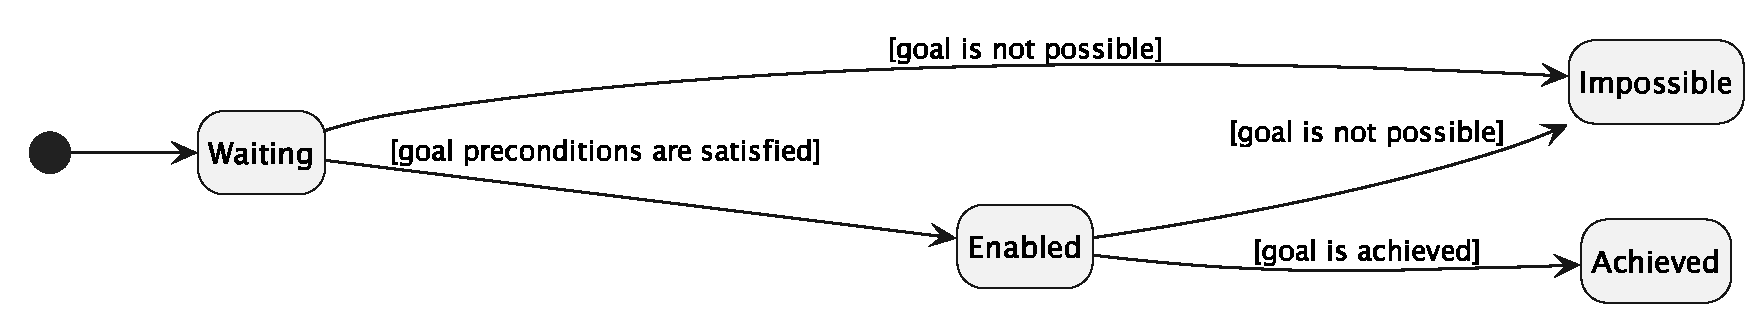
\includegraphics[width=\textwidth]{images/goal-life-cycle.eps}
    \caption{Goal life cycle.}
    \label{fig:goal-life-cycle}
\end{figure}

Each non-leaf goal is decomposed into subgoals by \textit{plans} using three operators:
\begin{itemize}
    \item \textit{sequence}: the plan $g1 = g2, g3$ means that the goal $g1$ is satisfied if and only if $g2$ and subsequently $g3$ are satisfied;
    \item \textit{choice}: the plan $g1 = g2 | g3$ means that the goal $g1$ is satisfied if one and only one of $g2$ or $g3$ is satisfied;
    \item \textit{parallel}: the plan $g1 = g2 \parallel g3$ means that the goal $g1$ is satisfied if both $g2$ and $g3$ are satisfied, and they can be pursued in parallel.
\end{itemize}
Therefore, a social plan denotes a structure of interrelated organizational goals to be satisfied by multiple agents that have to coordinate to handle dependencies between goals.


Goals can be gathered together in \textit{missions}, meaning that they should be achieved under the responsibility of a single agent.
When an agent participates in the organization, it commits to missions, meaning that it will try to achieve the goals contained in them.

All of the above concepts regarding functional abstractions are defined within a \textit{social scheme}, which denotes the collective and coordinated behavior that is expected to be produced by a group of agents in the organization.

\subsection{Normative Dimension}
Whereas structural abstractions address the structuring of the agents in the system and functional abstractions target the coordination of their behavior, normative abstractions are concerned with the regulation of agents' behavior in the organization

The main concept is the \textit{norm}, which defines the rights and duties of agents by connecting the structural and the normative dimensions with deontic modalities such as \textit{obligation}, \textit{permission}.
Specifically, a norm refers to a role and a mission, thus obliging or permitting the agent playing the role to commit to the mission.
Moreover, a norm can be associated with an \textit{activation condition} that must be satisfied in order for the norm to be active, and a \textit{time constraint} that defines a deadline by which the norm must be satisfied.

\subsection{Organization Execution}
As introduced in \cref{moiseplus}, the organization entity is a representation of the state of the organization at runtime which is distributed into three types of entities.
The concept is similar to the one of \textit{classes} and \textit{objects} in object-oriented programming.

The \textit{group entity} is related to a group defined in the structural specification and its state contains:
\begin{itemize}
    \item the owner of the group;
    \item the links to children and parent groups;
    \item the set of role-player agents with their links.
\end{itemize}

The \textit{scheme entity} is related to a social scheme defined in the functional specification, including:
\begin{itemize}
    \item the owner of the scheme;
    \item the groups responsible for the scheme;
    \item the commitments of the agents to the missions;
    \item the state of each goal.
\end{itemize}

Finally, the \textit{normative entity} is related to group and social scheme entities.
It is created every time a group entity becomes responsible for a scheme entity and it contains the status of a set of norms build from the abstract norms of the normative specification.

\section{Functional Requirements}
Since the platform needs to be compatible with \moise{}, the final user should be able to:
\begin{itemize}
    \item Define the structure of the organization, in particular:
    \begin{itemize}
        \item Define the roles that agents can play;
        \item Define the groups of the organization, with the possibility to nest them;
        \item Define which roles belong to which groups;
        \item Define the main links between roles;
    \end{itemize}
    \item Define the expected behavior of the agents, which means:
    \begin{itemize}
        \item Define the collective goals that agents should achieve;
        \item Define the dependencies among the goals;
    \end{itemize}
    \item Assign the collective goals to roles, thus connecting the structure and the behavior of the organization;
    \item Save and load the organizations they create for future editing;
    \item Enforce the organization they create on running agents.
\end{itemize}

\section{Non-Functional Requirements}
Given the target user of this platform, i.e. domain experts, the main non-functional requirement is the ease of use and user-friendliness.
In particular, the interface should be as clean as possible with a minimal set of easy-to-understand features so that users will not feel overwhelmed by it.

What is more, the system should be easily accessible.
Therefore, the most suitable technologies for its development are web-based ones, which allow the user to access the platform from any device with an internet connection.
Although, a mobile version is not required since it will mainly be used on wide screens.

The above functional and non-functional requirements, that arose from the \textit{IntellIoT} project and the need to address a higher level of abstraction for the definition of organization-centered MAS by domain experts, will be therefore fulfilled through the development of a visual programming language and a web-based integrated development environment that exploits it.